\chapter{Feedback Model}
The outputs of the system are the feedbacks to the detected postures. The candidate output devices can be classified into three groups. The first group includes the devices usually already put in the environment, such as television. The second group refers to the mobile devices that can be carried into the environment easily and frequently, such as smartphone, tablet, and laptop. The third group consists the output devices that are available to and support different functions provided by the ones proposed above from a list of output device (See Appendix~\ref{appendix:output_devices_list}) presented by Computer Help~\cite{output_device}, namely, projector, speaker, and printer. These devices could not only work individually, but could also cooperate with each other.

Besides the output device, another concern of the system is the intervention extent of the feedback. According to Dostal, Kristensson, and Quigley~\cite{estimate_viewing_distance}, the types of feedback can be divided into disruptive, obtrusive, subtle, and undetectable by its intervention extent. The subtle feedback is more preferred than the others as the system aims at improving the target postures while influencing users current activities at the least level. However, the intervention extent would be increased if a detected target posture were not successfully improved after the delivery of the feedback with less intervention extent. This is for preventing the harm that maintaining a bad posture might cause to the body. Therefore, the feedback candidate would be modeled with three intervention extents in the research, namely, subtle, subtle to obtrusive, and obtrusive. The disruptive feedback would be avoided as it could cause a strong negative user experience to the users and reduce the willingness for the application of the system of the users.

\section{Level 1 : Subtle}
A feedback can be divided into the informative type and the non-informative type. For the non-informative feedback candidate, the projectors would make the room slightly flicker, the volume of the speakers from every device within the environment would be decreased, and the display of the devices would be dimmed if a target posture were detected (See Figure~\ref{fig:brightnessChange}). The volume and the brightness are chosen as the feedback is due to their property of consistency: there is always a degree of the volume for a video and a degree of the brightness for displays. The users could perceive the change immediately once a bad posture is detected. Also, the users can detect the volume and brightness back to the normal right after the posture is improved.

\begin{figure}[h]
\centering
  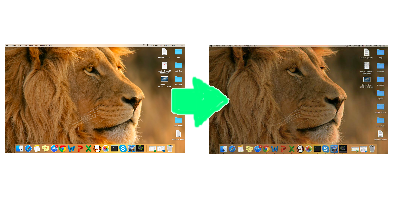
\includegraphics[width=0.5\textwidth]{figs/brightness}
\caption{Brightness of display Change in Level 1}
\label{fig:brightnessChange}
\end{figure}

The way could map the bad posture behaviour and a detectable effect without making a negative user experience. However, the non-informative feedback has two primary limitations. First, the users may simply adapt to the stimuli. Second, there is no explanation for the delivery of the feedback and the user might be confused about where the problem from. The first limitation could be overcome by providing other feedback with stronger intervention extent that the users could no longer easily ignore or adapt to, and the second limitation would require some informative feedback methods to be delivered in the mean time to overcome. The projectors could produce the animation of an elf (See Figure~\ref{fig:transparent_elf}), which has the abbreviation of \textit{Embedded Live-posture Feedback} on the wall, which show graphical indications about how to improve current posture. The indications would be illustrated in a relaxing tone with high degree of the transparency that decreases the extent of interference. Another method is to provide the spelling suggestions by the mobile device when a target posture is detected and the user is typing. The method presents the keywords related to the user’s current posture and therefore enhance the user’s awareness on it. The system would also switch the presentation of an input letter loceated close to the beginning letter of the keyword for current detected posture in the keyboard into the keyword’ beginning letter, therefor the keyword can be suggested. For examples, the system would suggest ``slouch'' when a user with a slouch posture types “s”, and it would also switch the presented letter as ``s'' even the user typed ”d” actually for the suggestion of ``slouch'' to be presented again. The index of the input letter, presented letter and the spelling suggestion is illustrated in Table~\ref{tab:input_letter_spelling_lvl1}. 

\begin{figure}[h]
\centering
  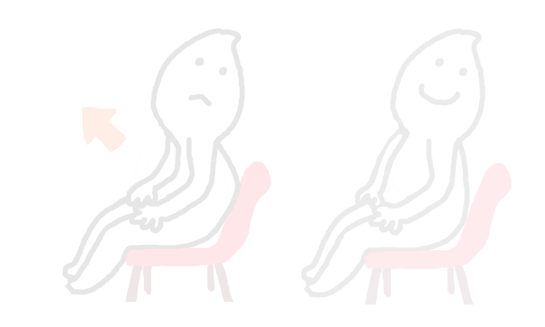
\includegraphics[width=0.5\textwidth]{figs/transparent1}
\caption{Sample Animation Illustration Decomposition}
\label{fig:transparent_elf}
\end{figure}

\begin{table}
\centering
\begin{tabular}{l c c l} 
\hline\hline
Condition & Input & Present & Suggestion Word\\
\hline\hline
General & B & B & body\\
  & P/O & P & posture/pain\\
  & H & H & health\\
  & S & S & sit/soreness\\
\hline
Lower back & B & B & back\\
not supported & L/K & L & lower-back\\
  & S & S & spine\\
\hline
 Slouch & B & B & back\\
  & S/A & S & spine/slouch\\
\hline
 Stationary & M & M & move\\
  & S & S & shake\\
  & W & W & wave\\
 (specific region) & A & A & arm\\
  & L & L & Leg\\ 
  & T & T & trunk\\
  & H/G & H & head\\
\hline
Bad viewing height/ & D & D & distance\\
distance  & E/W & E & eye/eye-care\\
  & N/M & N & neck/neck-tilt\\
  & S & S & sight\\
  & T & T & tilt\\
  & V & V & viewing-height\\
\hline
Cross Leg & C & C & cross-leg\\
  & L & L & leg\\
\hline\hline
\end{tabular}
\caption{Index of Input, Presented Letter, and Spelling Suggestions in Level 1}
\label{tab:input_letter_spelling_lvl1}
\end{table}

In addition, there are some feedback methods targeting a particular posture. The projector would produce the shadow on the top side of the furniture for a high viewing height posture, which is an implication showing the user is currently tilting his/her head and looking from bottomside up (See Figure~\ref{fig:hvh}). The colour of the shadow could change from time to time to be more fancy and avoid causing a sense of depression related to the colour of gray scale. The projector could also highlight the edge of the furniture to make the sense that the user is currently close to it to feedback a short viewing distance posture (See Figure~\ref{fig:svd}). 

\begin{figure}[h]
\centering
  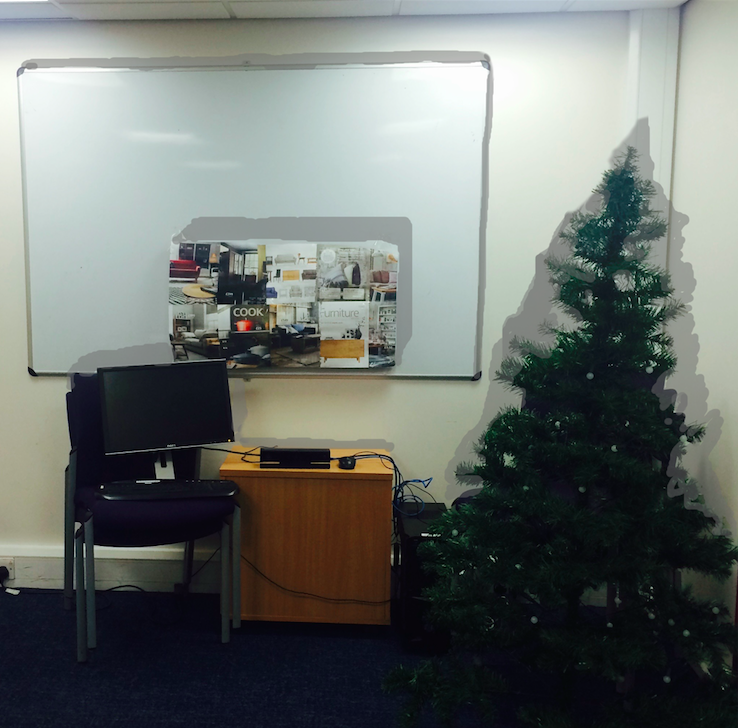
\includegraphics[width=0.5\textwidth]{figs/projector2in1}
\caption{Projector Feedback for High Viewing Height}
\label{fig:hvh}
\end{figure}

\begin{figure}[h]
\centering
  \includegraphics[width=0.5\textwidth]{figs/projector3in1}
\caption{Projector Feedback for Short Viewing Distance}
\label{fig:svd}
\end{figure}

To conclude, the design rationale behind the feedback in this level is to be noticeable but cause the least interference to the activities that the users are engaging in, and the provide a user experience which is not flat or annoying. The feedback methods in the level are summarised in Table~\ref{tab:feedback_model_lvl1}.

\begin{table}[h]
\centering
\begin{tabular}{l l l} 
\hline\hline
 Condition & TV + Mobile Devices & Projectors\\
\hline\hline
 &1. Decrease the volume & 1. Slightly flicker\\
Any bad posture &2. Dim the displays & \\
&3. Switch input letter and & \\
 & \ \ \ \ provide spelling suggestion & \\
\hline
 &  & 1. Provide animation \\
 & &2. High viewing height: \\
 && \ \ \ \ Project shadow for furniture\\
Specific posture&1. Switch input letter and & 3. Low viewing height:\\
  & \ \ \ \ provide spelling suggestion& \ \ \ \ Project shadow for furniture\\
  & & 4. Close viewing distance:\\
  & &\ \ \ \ Highlight furniture edge\\
\hline\hline
\end{tabular}
\caption{Feedback Model in Level 1}
\label{tab:feedback_model_lvl1}
\end{table}

\section{Level 2 : Subtle to Obtrusive}
The intervention extent of feedback would increase if the effect of the feedback in subtle level did show. The amplitudes of the methods used in level 1 would be increased and some new candidate methods in this level. The methods can be classified into two groups according to their targeting posture type, which are general and specific. A general feedback is provided using the projector to make an angle and a devil clock on the wall respectively counting the total duration that the user has bad postures and good postures (See Figure~\ref{fig:adc}). On the other hand, the mobile devices also support two feedback methods for general target postures. The first method is to increase the presentation priority of posture-related news or research on the social media, which could increase the possibility for the users to receive the related information and be aware of the need for posture improvement. The second method is to switch the original ring tone for the mobile phone to the theme song of the system. Both the melody and the lyrics could be helpful on reminding the users to improve the posture. 

\begin{figure}[h]
\centering
  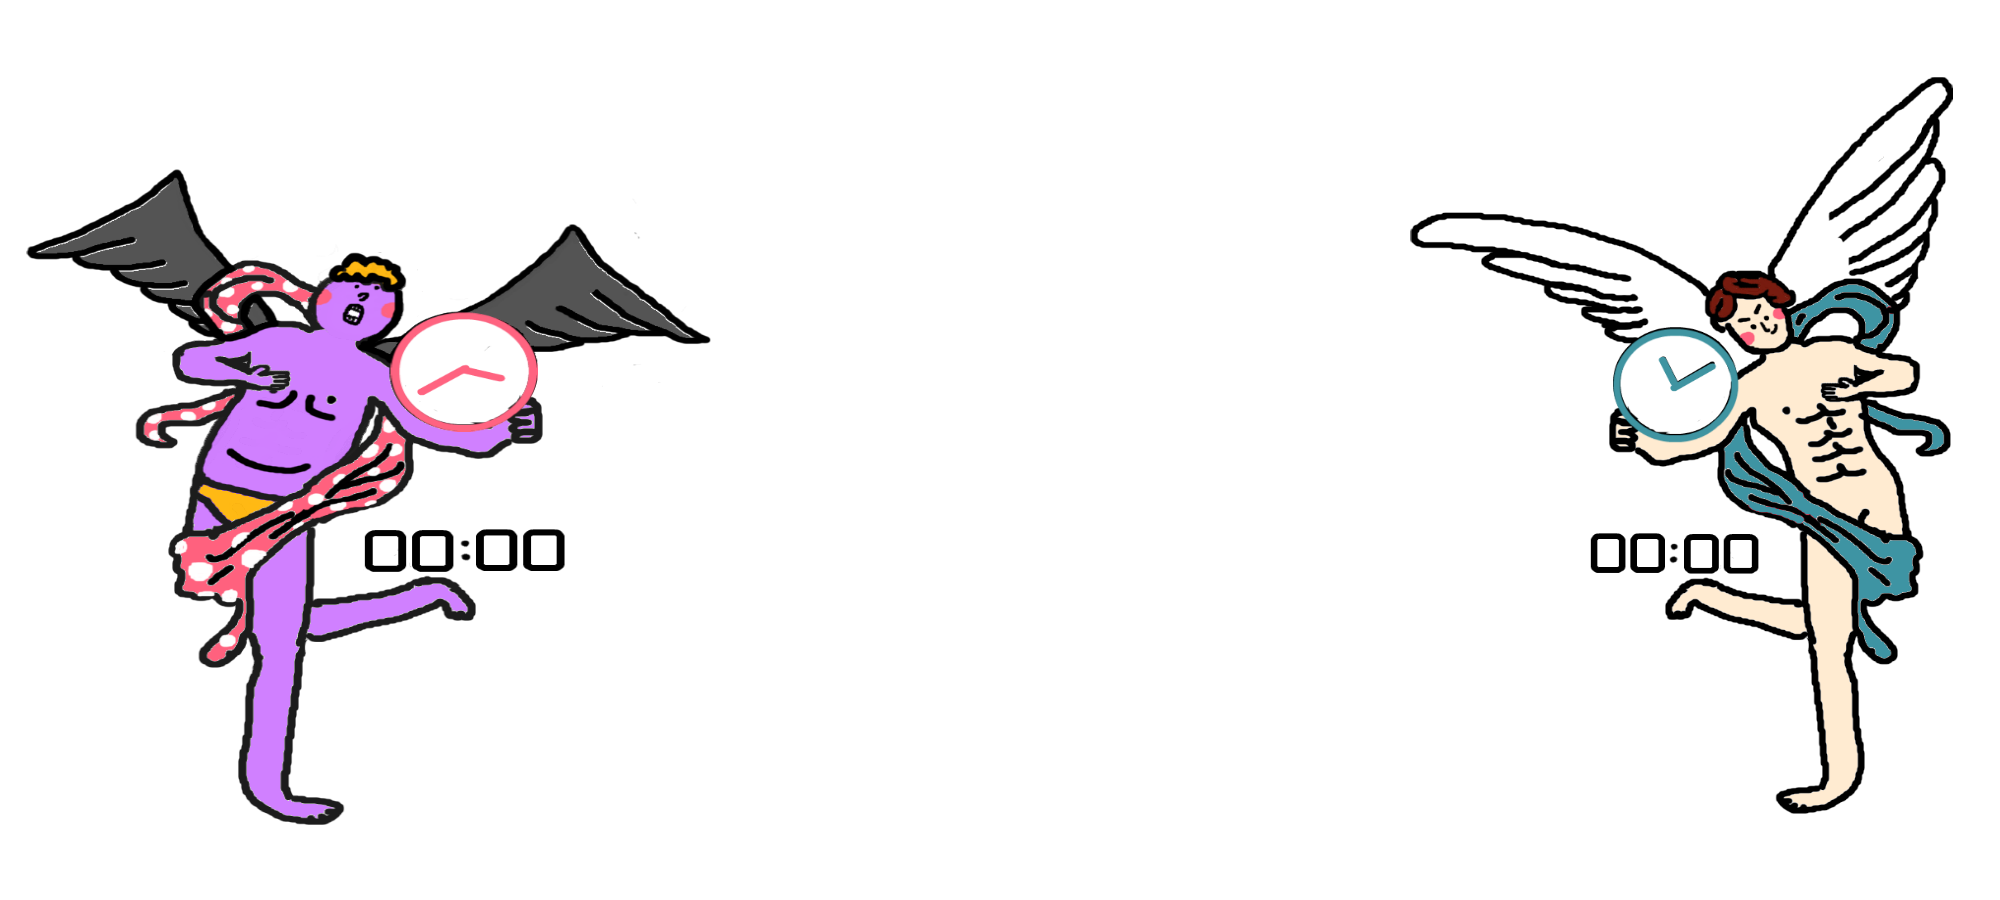
\includegraphics[width=0.5\textwidth]{figs/ad}
\caption{Angel and Devil Clock Feedback}
\label{fig:adc}
\end{figure}

For the feedback targeting a specific posture, the projector would make the effect as there is a starring sky on the ceiling, with shooting stars falling onto the floor to lead the sight of the users downwards for a high-viewing height posture, the starring sky would then fade away while some flowers grows up from the floor. The projector would also feedback to a low-viewing height posture by making some figures of the nestlings slowly fly upwards from the bush on the floor to lead the sight of the users upwards.

For the slouch or lower back not supported posture, the projector could provided the illusion that the room is slightly rotated against the x-axis to simulate the detected posture, by projecting the transformed picture in the same scale of the room. Same techniques could be used to provide feedback to a cross-leg posture, which is to make an illusion that the room rotated against the z-axis and the room’s centre of gravity perceived as moving towards to the opposite side of the upper leg. The sense of imbalance could make the user to put the upper leg down to try to make the sense of balance to the room returns.

If a stationary posture were detected, the projector would create the effect which looks like the furniture in the room is shaking and the dusts accumulated on the top of it are falling down, which implies that the user has kept stationary for too long even the dusts could be accumulated. The mobile device, on the other hand, would feedback to a short viewing distance posture by delivering a GPS-like notification to indicate the user how far he/she currently is from his/her supposed “destination” for a user with the posture.

There are some methods that could be applied to any target posture. First, the projectors could project a skeleton structure onto the wall, with the constrained joints due to the user’s current posture highlighted by different colour, bigger size, and flicker effect. Second, if the user were using an interface containing many words on the mobile device, the letters that consist the keyword related to the current posture would be subsequently highlighted. Third, the social media would be set to recommend some news or research related to the users current posture, helping the user to get more understanding about the impact it might cause and the need on improving it. Forth, an application could be developed on the mobile devices in the form of a messenger. The system would deliver the information, illustrated by animation with or without a voice effect, of current posture, and enable the interaction. 

The candidate methods can cooperate with each other to make the effect of the system more significant. The methods proposed in this level is summarised in Table~\ref{tab:feedback_model_lvl2}. 

\begin{table}
\centering
\begin{tabular}{l l l l} 
\hline\hline
 Condition && TV / Mobile Devices & Projectors\\
\hline\hline
General & &1. Decrease volume & 1. Flicker\\
 & &2. Dim displays &2. Angle clock / devil clock\\
& &3. Reset ring tone &\\
 & &4. Reset screen saver &\\
\hline
Specific & Common &1. Auto correct
inputs  & 1. animation presentation\\  
 & & 2. Recommend related news  & 2. animation guide\\
 & & 3. Send messages & \\
 & & (visual+audio+touch) &\\
 & & 4. Highlight keyword in text &\\
 & & 5. Skeleton impact highlight &\\
\hline
 & Viewing & & High viewing height:\\
 & height & & 1. shadows on the bottom\\
 & & & 2. starring sky animation\\
 & & & Low viewing height:\\
& & & 1. shadows on the top\\
 & & & 2. nestlings animation\\
\hline
&viewing & Deliver GPS notification &  Highlight and widen\\
& distance & & furniture edge\\
\hline
& Lower & & Illusions for room\\
 & back & & rotated against x-axis\\
\hline
& Slouch & & illusions for room\\
& & &  bent from x-axis\\
\hline
& Leg &&  Illusions for room\\
& crossed &&  rotated against z-axis\\
\hline
& Stationary & & Illusion for furniture\\
&&& shaking and dusts falling\\
\hline\hline
\end{tabular}
\caption{Feedback Model in Level 2}
\label{tab:feedback_model_lvl2}
\end{table}

\section{Level 3 : Obtrusive}
Some feedback methods in this level are modified using of the methods proposed in the prior levels. For example, the volume of the speakers as well as the brightness for the displays would be increased when a target posture is detected instead of decreased and dimmed. The design rationale behind this is to make the user not simply able to detect the change, but under higher stimuli as well. Also, the system would automatically correct some words beginning with the letter for the keyword of current detected target posture rather than simply suggest it, which makes the message less likely to be ignored. The index that indicates the details of the functions can be seen in Table~\ref{tab:feedback_model_lvl2}.


The other modifications from the previous methods include switching the mobile into outdoor mode, and the ring tone becoming the voice command for current posture improvement; making the projected shadow of furniture for a low viewing height or high viewing height posture dynamic, which can extends upwards or downwards; and the highlighted furniture edge feedback for the short viewing distance posture would flicker and wave.

There are also many new feedback methods proposed. First, the users would be asked by the system to present that they would make efforts on their posture improvement when they firstly use the system. The picture taken by the Kinect when the user mad promise could be projected onto the wall in this level, using the rationale of cognitive dissonance to remind the users to keep their behaviour consistent. They would tend to change the later action (having a bad posture) according to the prior action (making promise to have good posture for the goods of health) to avoid the anxiety caused by the cognitive dissonance. 

Secondly, a method inspired by the design of Half Room~\cite{half_room} (See Figure~\ref{fig:halfroom}) would be integrated with the feedback for cross-leg, lower back not supported and slouch posture. The position and the orientation of the half room are modified for each posture individually. This is for using the half room’s design rationale of anxiety avoidance and curiosity about the extending, to push the users to change current posture. For example, when there is a lower back not supportive posture, the half room picture would be projected and perceived parallel to the body, in which the user would change the posture to avoid the anxiety caused by the alignment and explore what could be shown in the blank.

\begin{figure}[h]
\centering
  \includegraphics[width=0.5\textwidth]{figs/halfroom}
\caption{Weighting for audio forms}
\label{fig:halfroom}
\end{figure}

Thirdly, some 3D objects could be projected on the area close to the display to make a crowding sense for user having a short viewing distance posture. At last, the printer could automatically colour print the picture of the user with his/her current posture, along with the description of the duration of current posture, the impact it might cause to the body, and the relevant research on it. It could be a powerful method to instruct the user about what should be understood about the user. 
The cooperation between multiple methods in the level is presented in Table~\ref{tab:feedback_model_lvl3}. 

\begin{table}
\centering
\begin{tabular}{l l l l} 
\hline\hline
 Condition && TV / Mobile Devices & Projectors\\
\hline\hline
General & &1. Decrease volume & 1. Flicker\\
 & &2. Dim displays &2. Angle clock / devil clock\\
& &3. Reset ring tone &3. project promising picture\\
 & &4. Reset screen saver &\\
\hline
Specific & Common &1. Auto correct
inputs  &1. animation presentation\\  
 & &2. Recommend related news  & 2. animation guide\\
 & &3.Send messages & \\
 & &  (visual+audio+touch) &\\
 & &4. Highlight keyword in text &\\
&&  5. elf reminder on &\\
& &  background/browser homepage & \\
& &6. Color print & \\
& &  current pics with &\\
&&  description &\\
& &7. Reser ring tone &\\
& & using voice command & \\
& & 8. Skeleton impact highlight& \\
\hline
 & Viewing & & High viewing height:\\
 & height & & 1. shadows on the bottom\\
 & & & 2. starring sky animation\\
 & & & 3. half room\\
 & & & Low viewing height:\\
& & & 1. shadows on the top\\
 & & & 2. nestlings animation\\
 & & & 3. half room\\
\hline
&Viewing & Deliver GPS notification &1. Highlight and widen\\
& distance & &  furniture edge\\
& & & 2. Make 3D objects full\\ 
\hline
& Lower & &1. Illusions for room\\
 & back & &  rotated against x-axis\\
 & & & 2. Half room\\
\hline
& Slouch & &1. Illusions for room\\
& & &  bent from x-axis\\
 & & & 2. Half room\\
\hline
& Leg && 1. Illusions for room\\
& crossed &&  rotated against z-axis\\
 & & & 2. Half room\\
\hline
& Stationary & & illusion for furniture\\
&&& shaking and dusts\\
&&& falling\\
\hline\hline
\end{tabular}
\caption{Feedback Model in Level 3}
\label{tab:feedback_model_lvl3}
\end{table}

\section{Summary}
The model aims at discussing various ways to provide feedback to the detected postures. 10 candidate methods are proposed in level 1, while 20 methods are proposed in level 2 and 33 methods in level 3. The structure of the model is illustrated in Figure~\ref{fig:feedback_model_2}. The colours are used to encode the targeting posture types, and the presentation of the gradient background of a feedback method indicates that the intervention extent of the method would become increase if the improvement of the target posture were not observed. 

\begin{figure}[h]
\centering
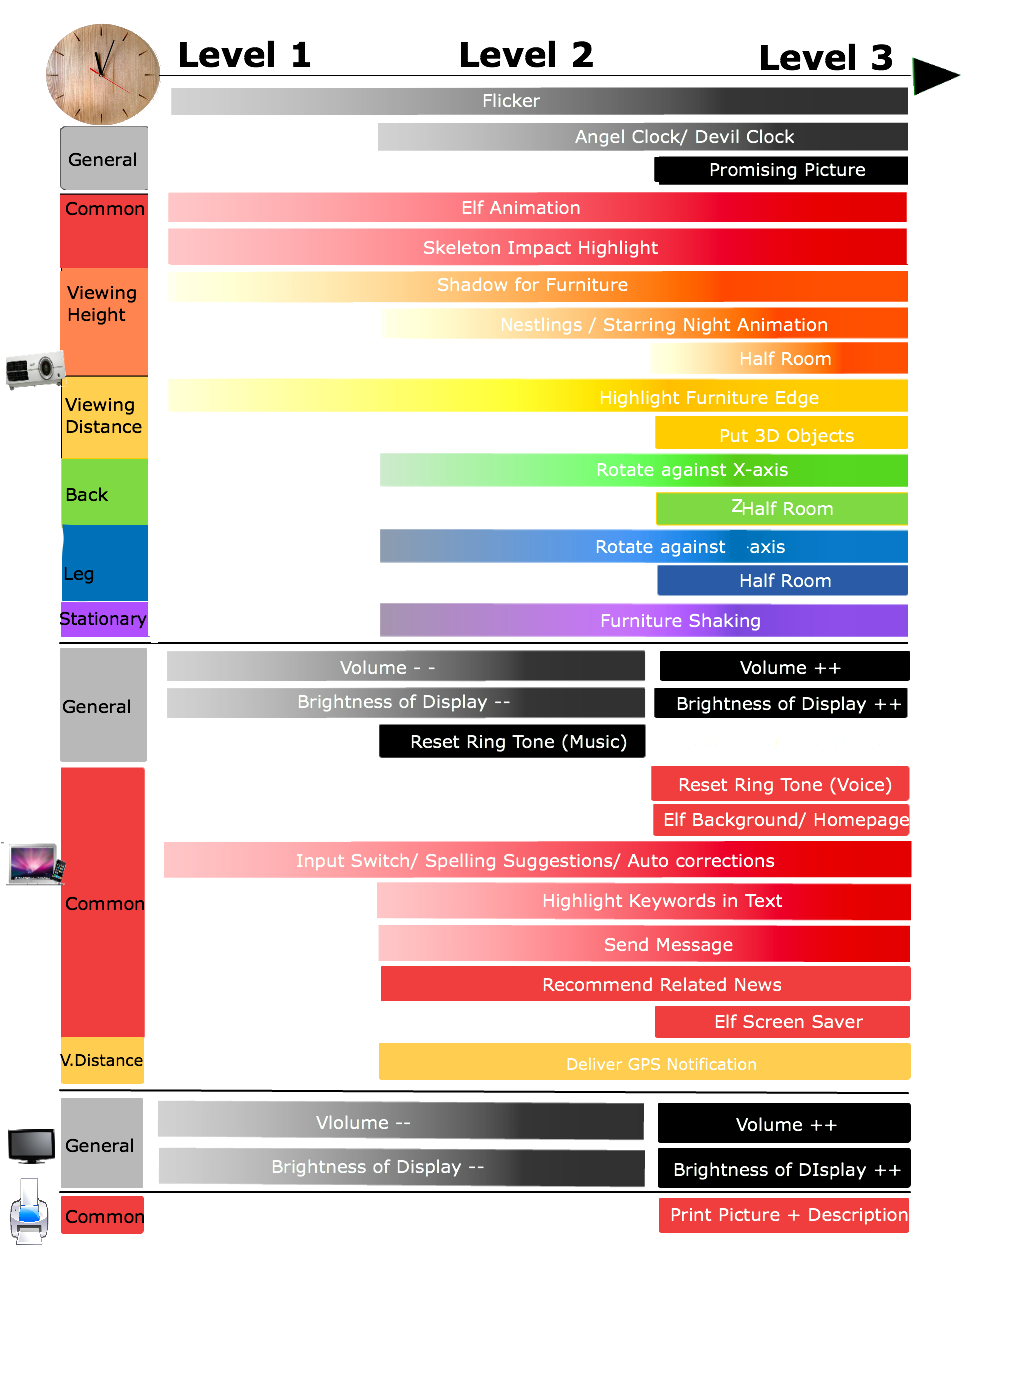
\includegraphics[width=1\textwidth]{figs/feedbackmodel2}
\caption{Feedback Model}
\label{fig:feedback_model_2}
\end{figure}
